\chapter{はじめに}
% \chapter{卒業論文の作成と発表の手順}
\thispagestyle{myheadings}

% 卒業研究は1名（個人）または2〜4名のグループで行う．卒業研究を行う個人
% またはグループは以降に示すようにレジュメの執筆，本論文の執筆，口頭発表
% を行わなければならない．なお，グループで卒業研究を行う場合は，グループ
% で1件，執筆，発表等を行うことになる．

% \section{スケジュール}
\section{背景}
\label{sec:schedule}
対面でのインフォーマルなコミュニケーションは組織内の関係構築や業務効率の向上において重要な役割を担うとされている\cite{inf}．
例えば，日常的な雑談や立ち話を通じて業務の進捗や課題が共有され，正式な会議や調整の負担が軽減される場合がある．
また，こうしたやり取りを通じて心理的距離が縮まると，相談や協力を行いやすい関係性が形成されると考えられる．
一方で，このような対面コミュニケーションの重要性が指摘される中，近年はリモートワークの普及や柔軟な勤務形態の導入により，人々が同じ場所・同じ時間帯に集まる環境を前提とした働き方が変化しつつある．
このような環境の変化は対面コミュニケーションの発生にも影響を与え，従来のような偶発的な対面に依存した関係構築が十分には成立しにくくなっていると考えられる．


%
近年の働き方の変化の一例として，全面的なリモートワークからハイブリッドワークに移行する傾向が見られ，オフィスに出社する機会が再び増加している点が挙げられる．
国土交通省が公開する資料\cite{tel}によると，令和4年度から令和5年度にかけて全国の雇用型ワーカーの割合が26.1\%から24.8\%と減少傾向にある．
COVID-19の流行が始まった令和1年度よりも高い水準ではあるものの，出社回帰の傾向にあると言える．
また，テレワークの実施頻度が週5〜7日の雇用型テレワーカーの割合は18.7\%から17.7\%と減少傾向にある一方で，テレワークの実施頻度が週1〜4日の雇用型テレワーカーの割合は，53.7\%から58.1\%と増加傾向にある．
これは出社とテレワークを組み合わせたハイブリッドワークを実施している労働者の割合が拡大傾向にあると言える．
このような働き方では出社の有無や頻度が個人ごとに異なる形で分散しており，従来のように全員が同じ時間帯に在室する状況は減少している．

%
また，柔軟な働き方を認める制度の普及により，個人の行動や滞在時間が多様化している点も，対面コミュニケーションの在り方に影響を与えている．
厚生労働省が公開する資料\cite{fle}によるとフレックスタイム制と通常勤務日を組み合わせる制度について「あってもよい」と考える労働者の割合は35.4\%と最も多い．
これはフレックスタイム制をはじめとする柔軟な勤務制度に対する潜在的な需要の大きさを示しており，個人が出社時刻や帰宅時刻を調整できる働き方が今後さらに広がる可能性がある．
しかし，このような柔軟性の高い環境では行動のタイミングが揃いにくく，対面機会は必ずしも十分に活用されていない．

%
これに伴い，対面機会を効果的に活用するためのコミュニケーション支援の重要性が高まっている．
滞在時間が個人ごとに分散する環境では偶発的な対面が生じにくく，特定のタイミングに着目した支援が求められる．
その中でも在室時のコミュニケーションは業務との関連付けが容易であるだけでなく，滞在時間の大部分がコミュニケーションの発生し得る時間帯に該当し継続的に観測・支援しやすいため，これまで多くの研究が在室時の場面を対象としてきた．
一方で，退室時の行動は業務外の時間と捉えられやすく，時間的にも限定的であるため，研究や支援の対象として十分に検討されてこなかった．

% スケジュールはL-Cam等を使って連絡されるので注意する．
% \begin{description}
%   \itemindent=1zw
%   \itemsep=0mm
%   \parsep=0mm
%   \item[*月**日(*)] タイトル提出
%   \item[*月**日(*)] レジュメ提出
%   \item[*月**日(*)] 卒業論文締切
%   \item[*月**日(*)] 卒業論文・制作発表会
% \end{description}


% \section{レジュメの提出}
\section{目的とアプローチ}
\label{sec:abstract}

本研究の目的は滞在者に帰路の一部を共にさせ，インフォーマルなコミュニケーションの発生を通じた組織内の関係構築の支援である．
退室時は作業が一区切りついて心理的に余裕が生まれ，誰かと同行する場合は関わる人数が限られる点も重なって気軽な会話が生じやすいと考えられる．
さらに，建物を出て公共交通機関に乗車するまでの移動時間においても会話が継続しやすく，一定のコミュニケーション時間を確保できる．
このような特徴から，退室時の同行はインフォーマルなコミュニケーションが発生しやすい状況であると考えられる．

%
しかし，退室時に他者を誘う行為には心理的な負担が伴う．
例えば，自身の作業を切り上げる適切なタイミングを見失っている場合には自分の帰宅時刻を明示できない.
そのため，その不確実な状態で他者を誘う行為が難しくなる．
また，誘った後に自身の作業が想定以上に長引いた場合には相手を待たせてしまう可能性があるので，声かけをためらう要因となる．
他にも，相手が他の活動や会話に関与している場合にはその行動を中断させてしまう懸念から声をかけにくくなると考えられる．
このような心理的要因から，本来であれば同行可能な状況であっても退室時の声かけが行われにくい可能性がある．

%
そこで本研究では，退室行動の中でも帰宅に至るタイミングに着目し，図\ref{fig:overview}に示すようなシステム，leaving-matchを提案する．
複数の滞在者が共に帰宅できそうな時刻(以下帰宅推奨時刻)をバスの発車時刻と組み合わせて提示する．
これにより，ユーザは自ら他者に声をかけなくても，一緒に帰れそうなタイミングを把握できる．
結果として，退室の判断や声かけに伴う心理的負担を軽減し，同行を選択しやすくなると期待される．
このような情報提示を通じて，帰宅時にコミュニケーションを発生させるきっかけの提供を目指す．

\begin{figure}[htb]
  \centering
  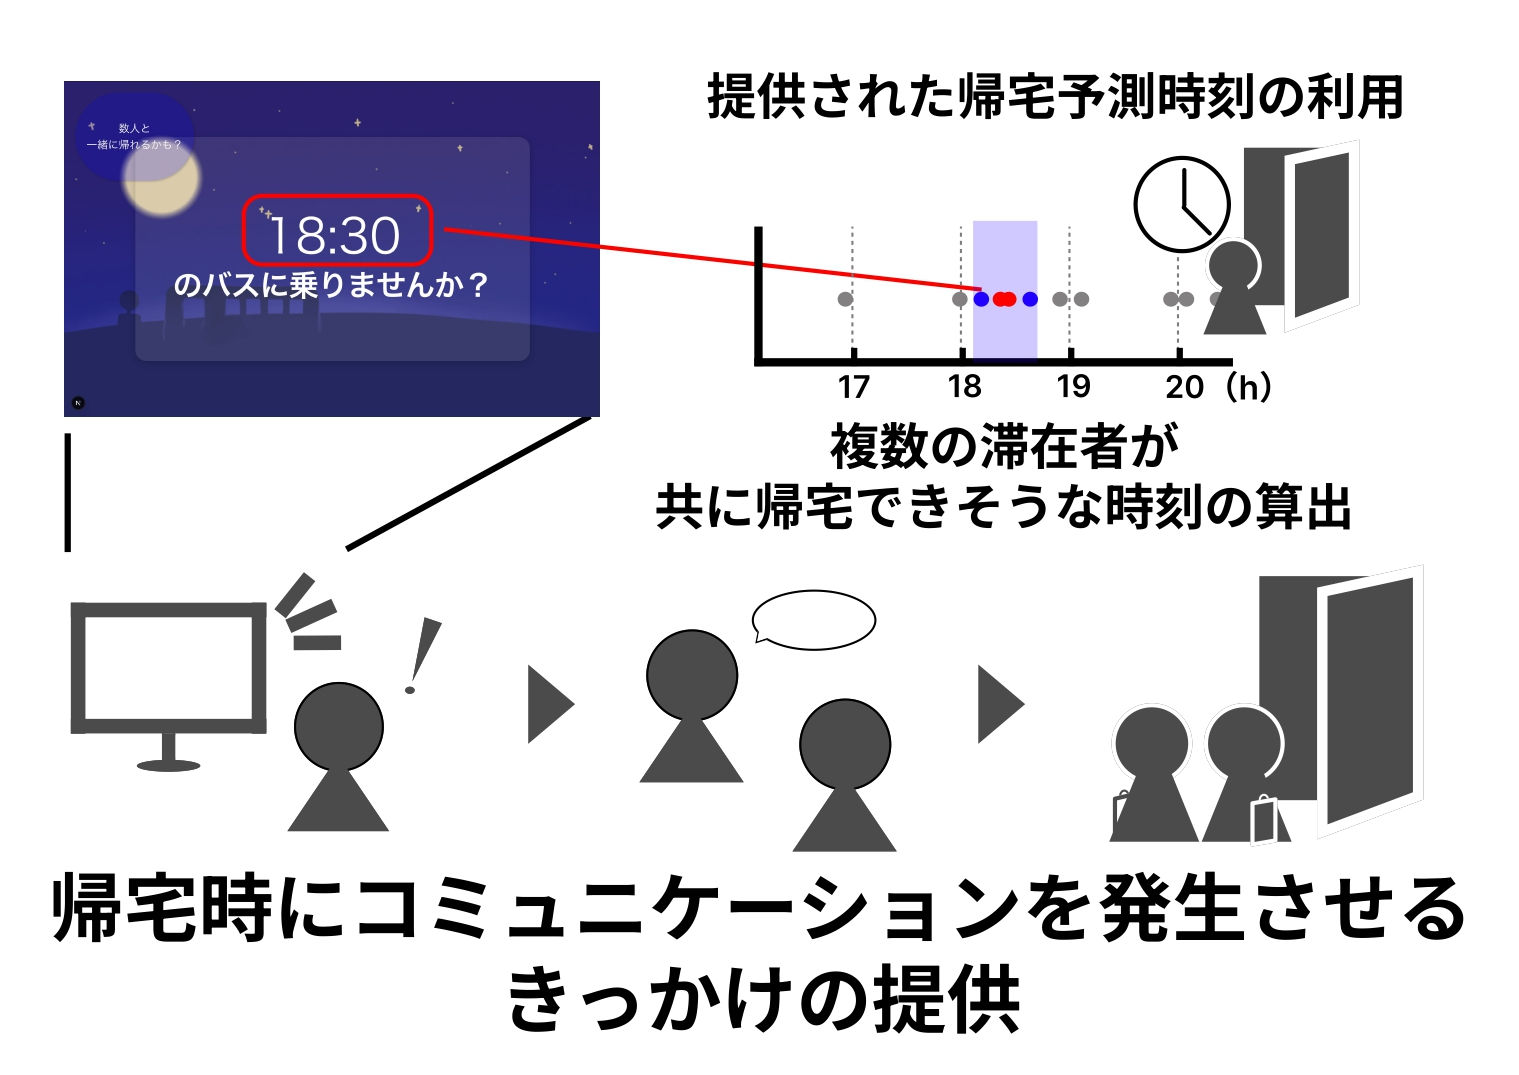
\includegraphics[width=0.8\linewidth]{fig/overview.jpg} % suzuki
  \caption{本研究の概要}
  \label{fig:overview}

\end{figure}

% 先に示した締切にしたがって，卒業研究の要旨を記したものを提出する．これ
% をレジュメという．レジュメは，指導教員の校閲を受け，提出許可を受けてか
% ら，指導教員経由で電子的に提出する．

% レジュメは，A4サイズにて提出し，印刷されて，\ulinej{審査にあたる各教員
%   と4年生及び各研究室に配布される．口頭発表時には，教員や聴講している学生は
%   このレジュメを見ながら質問をする．}
% よく推敲して，研究の要旨を充分に伝えられるものに仕上げる．
% 指導教員から提出を認められるまで，何度でも書き直す．
% レジュメの作成にあたっては \LaTeX やWordなどのソフトウェアを使用する．

% \section{卒業論文提出}
\section{論文構成}
\label{sec:thesis}


本稿の構成を以下に示す．
2章では，関連する分野の研究や事例を述べる．
3章では，先行研究である在室予測の提供を行うシステムとその基盤となる在室管理システムについて述べる．
4章では，提案する帰宅同行支援システムについて，詳細設計を述べる．
5章では，本研究で提案するシステムの有効性を確認するために行った実証実験の結果と考察を述べる．
最後に6章では，本研究についてまとめると共に今後の展望を述べる．

% 卒業研究の成果は，指導教員の指示に従って，論文の形式にまとめ，それを必
% 要部数製本する(通常2部)．論文は，情報科学科事務室に1部提出する．
% 提出された論文は，専攻で審査に使われた後，各教員の元で永年にわたって保
% 存される．卒業論文の提出にあたっては，レジュメの場合と同様に，指導教員
% の校閲を受け，また認印を(内表紙に)受ける．

% 卒業論文のおおよその書式は第2章で説明するが，各研究室のスタイルに従え
% ば良い．\LaTeX を利用する場合は，このマニュアルの\LaTeX ソースをテンプレー
% トと利用しても良い．

% \section{卒業研究口頭発表}
% \label{sec:presentation}

% 卒業研究の仕上げは，卒業研究口頭発表である．卒業研究を1人で行っている
% 人は個人で，2人以上のグループで行っている人はグループで発表する．
% 口頭発表は，公開制であり，1〜3年生の聴講も許されている．

% 口頭発表技術は，話し方，資料のまとめ方，印象的な資料の提示方法等も含む．
% 口頭発表技術を，ぜひこの機会を利用して習得して欲しい．発表はプレゼンテー
% ションソフトを利用して，ノートパソコンと液晶プロジェクターの組み合わせ
% で効果的な発表を行う．発表時間は次を基準とする．\\

% \begin{tabular}[h]{ll}
%   1人で発表を行う場合   & 10分(質疑応答3分を含む) \\
%   グループで発表を行う場合 & 15分(質疑応答5分を含む) \\
% \end{tabular}

% \section{卒業研究の審査・単位認定について}
% \label{sec:referee}
% 審査は論文，レジュメ，口頭発表および日常の研究態度を総合して行われる．

% Local Variables: 
% mode: japanese-LaTeX
% TeX-master: "root"
% End: 
